\documentclass{ximera}
\graphicspath{{./auto_generated_text/Week2MultivariableFunctionsandGraphing/graphics/}{./graphics/}}
\title{Practice Problems}
\begin{document}
\begin{abstract}
\end{abstract}
\maketitle
\section{Online Problems}
\begin{problem}
Consider the function $f:\mathbb{R}^2\rightarrow\mathbb{R}$ given by
\[
f(x,y) = x^2+4y^2 -2.
\]
What is the domain of $f$?
\begin{multipleChoice}
\choice{$\mathbb{R}$}
\choice{$\mathbb{R}\setminus \{0\}$}
\choice{$[0,\infty)$}
\choice{$(0,\infty)$}
\choice[correct]{$\mathbb{R}^2$}
\choice{$\mathbb{R}^2\setminus\{(0,0)\}$}
\end{multipleChoice}

What is the range of $f$?
\[
\textrm{Range }f = \answer{[-2,\infty)}
\]

Is $f$ onto?
\begin{multipleChoice}
\choice{yes}
\choice[correct]{no}
\end{multipleChoice}

\begin{problem}
We would like to restrict the codomain of the function $f$ so that it becomes onto. We'll describe our new codomain as the set of numbers $a$ in $\mathbb{R}$ such that some condition holds. Which condition gives us the largest possible codomain such that $f$ is onto?
\begin{multipleChoice}
\choice{$a\in\mathbb{R}$}
\choice{$a \geq 0$}
\choice{$a > 0 $}
\choice{$a\neq 0$}
\choice{$a = 0$}
\choice{$a \geq 2$}
\choice{$a > 2 $}
\choice{$a\neq 2$}
\choice{$a = 2$}
\choice[correct]{$a \geq -2$}
\choice{$a > -2$}
\choice{$a\neq -2$}
\choice{$a = -2$}
\end{multipleChoice}
\end{problem}

Is $f$ one-to-one?
\begin{multipleChoice}
\choice{yes}
\choice[correct]{no}
\end{multipleChoice}

\begin{problem}
We would like to restrict the domain of the function $f$, so that it becomes one-to-one. We'll describe our new domain as the set of points $(x,y)$ in $\mathbb{R}^2$ such that some condition(s) hold. Which condition(s) give us the largest possible domain such that $f$ is one-to-one?
\begin{selectAll}
\choice{$x\neq 0$}
\choice[correct]{$x\geq 0$}
\choice{$x > 0$}
\choice{$y\neq 0$}
\choice[correct]{$y\geq 0$}
\choice{$y > 0$}
\end{selectAll}
\end{problem}
\end{problem}

\begin{problem}
Let $f:\mathbb{R}^3\rightarrow\mathbb{R}^3$ be the function defined by
\[
f(\vec{x}) = 3\vec{x} + \textbf{i} - 2\textbf{j}.
\]

Find the component functions of $f$ in terms of $x$, $y$, and $z$.
\begin{align*}
f_1(x,y,z) &= \answer{3x+1}\\
f_2(x,y,z) &= \answer{3y-2}\\
f_3(x,y,z) &= \answer{3z}
\end{align*}
\end{problem}

\begin{problem}
Consider the linear function $f:\mathbb{R}^3\rightarrow\mathbb{R}^2$ given by $f(\vec{x}) = A\vec{x}$, where
\[
A = \left(\begin{array}{ccc}
1&5&2\\
-2&0&1
\end{array}\right),
\]
and $x = \left(\begin{array}{c}x_1\\x_2\\x_3\end{array}\right)$.

\begin{enumerate}
\item Determine the component functions of $f$ in terms of $x_1$, $x_2$, and $x_3$.
\begin{align*}
f_1(x_1,x_2,x_3) &= \answer{x_1 + 5x_2 + 2x_3}\\
f_2(x_1,x_2,x_3) &= \answer{-2x_1 + x_3} 
\end{align*}
\item Is $f$ one-to-one?
\begin{multipleChoice}
\choice{Yes}
\choice[correct]{No}
\end{multipleChoice}
\item Is $f$ onto?
\begin{multipleChoice}
\choice[correct]{Yes}
\choice{No}
\end{multipleChoice}
\end{enumerate}
\end{problem}

\begin{problem}
Consider the function
\[
f(x,y) = xy.
\]
What is the shape of the level curve at height $0$ of $f$?
\begin{multipleChoice}
\choice{Empty}
\choice{A single line}
\choice[correct]{Two intersecting lines}
\choice{Two parallel lines}
\choice{Circle}
\choice{Ellipse}
\choice{Parabola}
\choice{Hyperbola}
\end{multipleChoice}

What is the shape of the level curve at height $1$ of $f$?
\begin{multipleChoice}
\choice{Empty}
\choice{A single line}
\choice{Two intersecting lines}
\choice{Two parallel lines}
\choice{Circle}
\choice{Ellipse}
\choice{Parabola}
\choice[correct]{Hyperbola}
\end{multipleChoice}

What is the shape of the level curve at height $-1$ of $f$?
\begin{multipleChoice}
\choice{Empty}
\choice{A single line}
\choice{Two intersecting lines}
\choice{Two parallel lines}
\choice{Circle}
\choice{Ellipse}
\choice{Parabola}
\choice[correct]{Hyperbola}
\end{multipleChoice}

What is the shape of the level curve at height $2$ of $f$?
\begin{multipleChoice}
\choice{Empty}
\choice{A single line}
\choice{Two intersecting lines}
\choice{Two parallel lines}
\choice{Circle}
\choice{Ellipse}
\choice{Parabola}
\choice[correct]{Hyperbola}
\end{multipleChoice}

Which of the following is the graph of $f$?

\begin{image}
\begin{tikzpicture}
\node[inner sep=0pt] at (0,0)
    {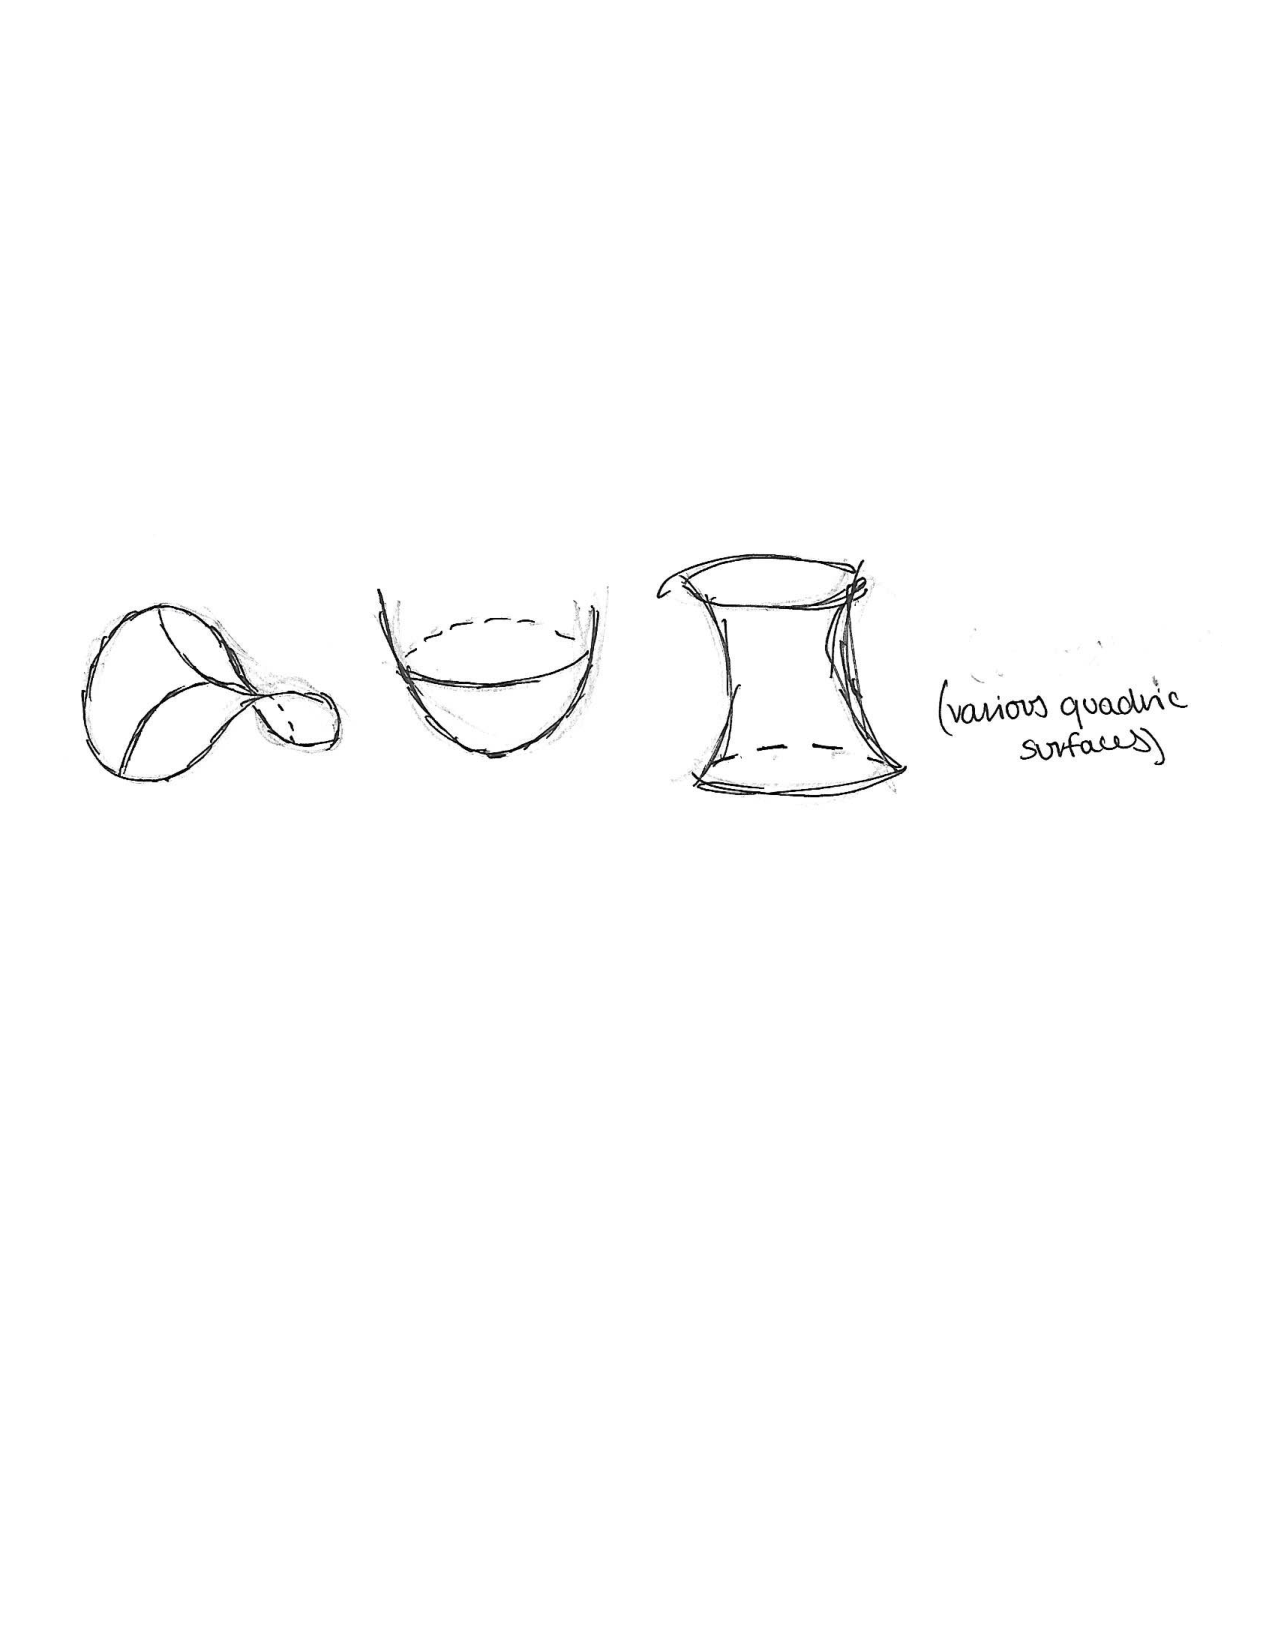
\includegraphics{quadric_options}};
\end{tikzpicture}
\end{image}
\end{problem}

\begin{problem}
Consider the function
\[
f(x,y) = |x|.
\]
What is the shape of the level curve at height $0$ of $f$?
\begin{multipleChoice}
\choice{Empty}
\choice[correct]{A single line}
\choice{Two intersecting lines}
\choice{Two parallel lines}
\choice{Circle}
\choice{Ellipse}
\choice{Parabola}
\choice{Hyperbola}
\end{multipleChoice}

What is the shape of the level curve at height $1$ of $f$?
\begin{multipleChoice}
\choice{Empty}
\choice{A single line}
\choice{Two intersecting lines}
\choice[correct]{Two parallel lines}
\choice{Circle}
\choice{Ellipse}
\choice{Parabola}
\choice{Hyperbola}
\end{multipleChoice}

What is the shape of the level curve at height $-1$ of $f$?
\begin{multipleChoice}
\choice[correct]{Empty}
\choice{A single line}
\choice{Two intersecting lines}
\choice{Two parallel lines}
\choice{Circle}
\choice{Ellipse}
\choice{Parabola}
\choice{Hyperbola}
\end{multipleChoice}

What is the shape of the level curve at height $2$ of $f$?
\begin{multipleChoice}
\choice{Empty}
\choice{A single line}
\choice{Two intersecting lines}
\choice[correct]{Two parallel lines}
\choice{Circle}
\choice{Ellipse}
\choice{Parabola}
\choice{Hyperbola}
\end{multipleChoice}

Which of the following is the graph of $f$?

\begin{image}
\begin{tikzpicture}
\node[inner sep=0pt] at (0,0)
    {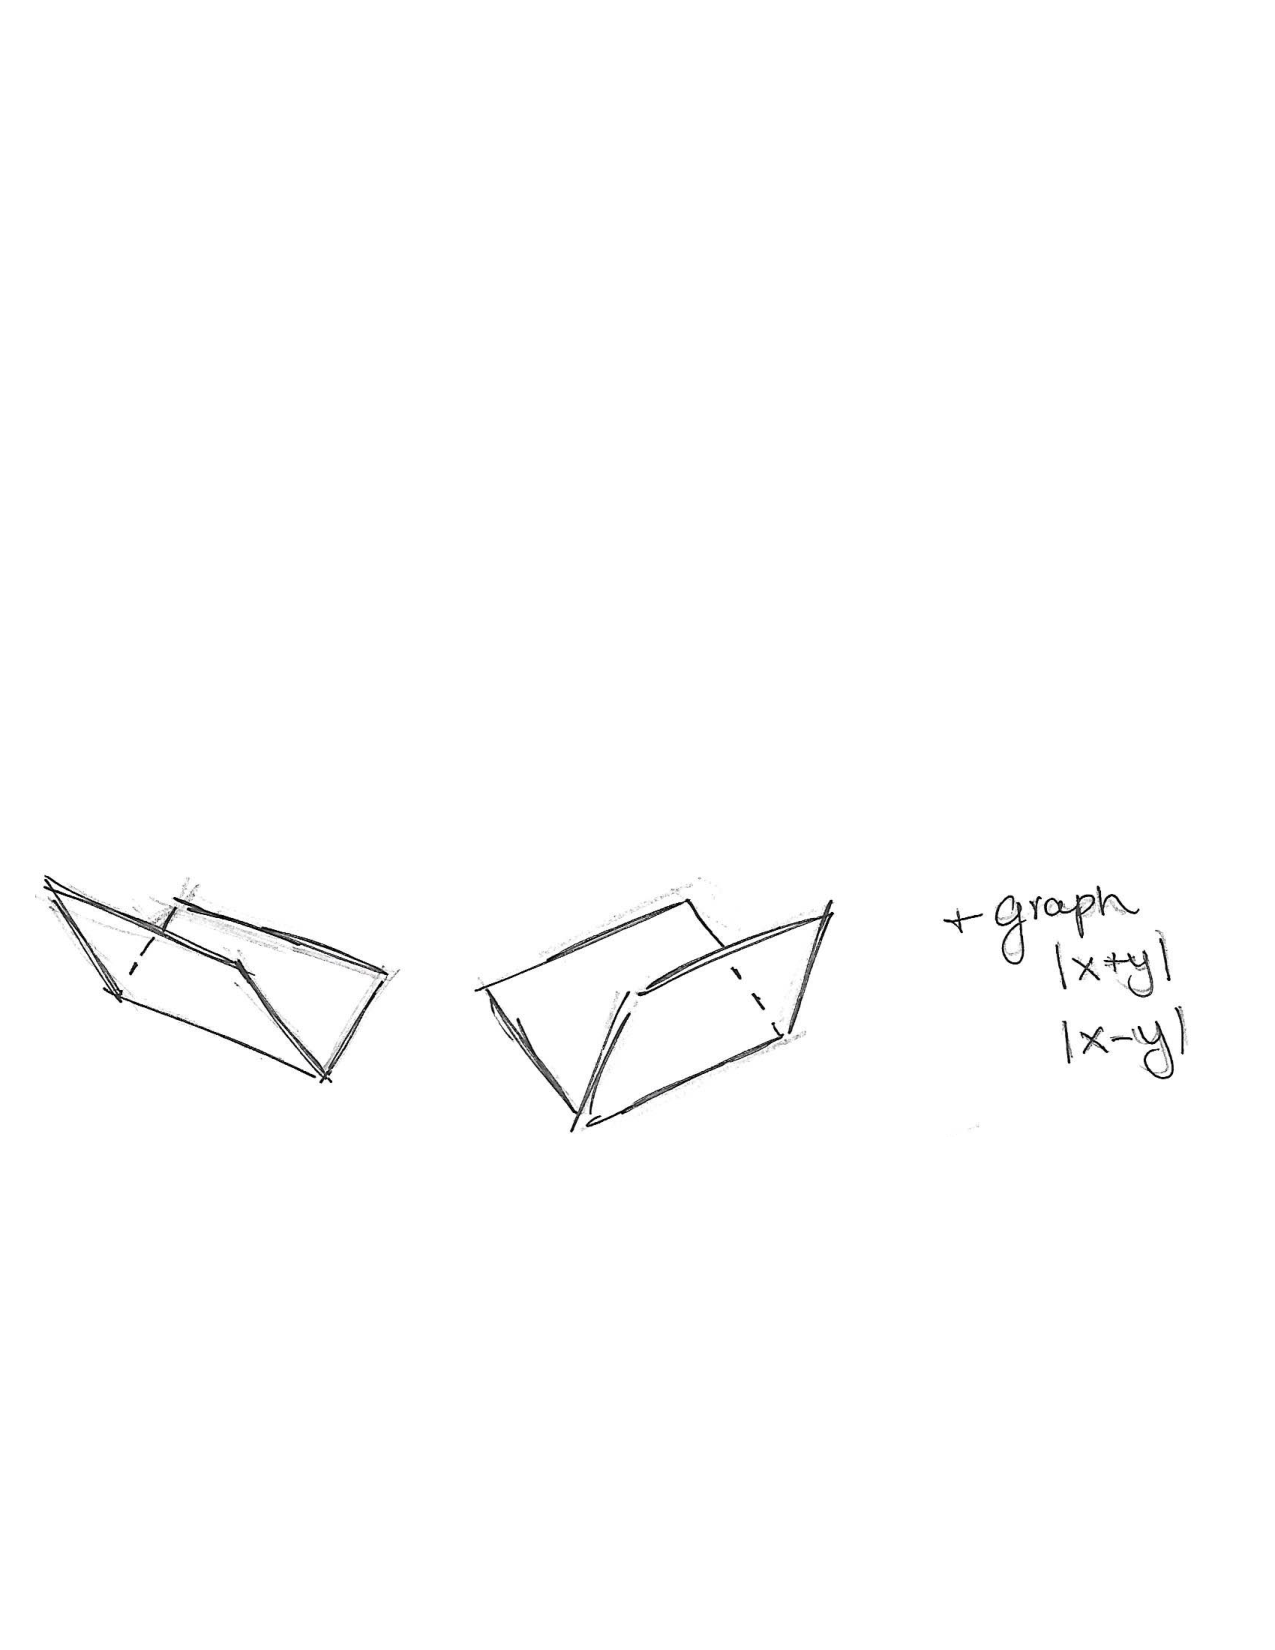
\includegraphics{wedge_options}};
\end{tikzpicture}
\end{image}
\end{problem}

\begin{problem}
Which of the following is the graph of the ellipsoid
\[
\frac{x^2}{9}+ y^2 + \frac{z^2}{4} = 1?
\]

PICTURES

Is there a function $f(x,y)$ such that the graph of $f$ is the ellipsoid above?
\begin{multipleChoice}
\choice{Yes}
\choice[correct]{No}
\end{multipleChoice}

\begin{problem}
Why is this impossible?
\begin{multipleChoice}
\choice{It wouldn't be one-to-one.}
\choice{It wouldn't be onto.}
\choice{There would be multiple inputs with the same output.}
\choice[correct]{A single input would need to have two outputs.}
\end{multipleChoice}
\end{problem}

\end{problem}

\begin{problem}
Classify the quadric surface defined by the equation
\[
x^2 + 4y^2 + z^2 + 8y = 0.
\]

\begin{multipleChoice}
\choice[correct]{Ellipsoid}
\choice{Elliptic Paraboloid}
\choice{Hyperbolic Paraboloid}
\choice{Elliptic Cone}
\choice{Hyperboloid of One Sheet}
\choice{Hyperboloid of Two Sheets}
\end{multipleChoice}

It is centered at $\answer{(0,-1,0)}$.

\begin{problem}
Which of the following is the graph of the quadric surface given above?

GRAPHS
\end{problem}


\end{problem}

\begin{problem}
Classify the quadric surface defined by the equation
\[
2x^2 + 2y^2 - 8y - z + 4 = 0
\]

\begin{multipleChoice}
\choice{Ellipsoid}
\choice[correct]{Elliptic Paraboloid}
\choice{Hyperbolic Paraboloid}
\choice{Elliptic Cone}
\choice{Hyperboloid of One Sheet}
\choice{Hyperboloid of Two Sheets}
\end{multipleChoice}

It is centered at $\answer{(0,2,-4)}$.

\begin{problem}
Which of the following is the graph of the quadric surface given above?

GRAPHS
\end{problem}


\end{problem}

\section{Written Problems}
\begin{problem}
Consider the function
\[
f(x,y,z) = \frac{4}{\sqrt{9-x^2-y^2-z^2}}.
\]
\begin{enumerate}
\item What is the domain of $f$? Describe this domain as a region in $\mathbb{R}^3$.
\item What is the range of $f$?
\end{enumerate}
\end{problem}

\begin{problem}
Consider the function 
\[
f(x) = x^2 + y^2 - 4.
\]
\begin{enumerate}
\item Draw at least five level curves of $f$.
\item Use these level curves to sketch the graph of $f$.
\end{enumerate}
\end{problem}

\begin{problem}
Draw the graph of the surface in $\mathbb{R}^3$ determined by the equation
\[
x = y^2/4 - z^2/9.
\]
Use level curves and/or sections to justify why your drawing is correct.
\end{problem}

\end{document}